%%%%%%%%%%%%%%%%%%%%%%%%%%%%%%%%%%%%%%%%%
% Simple Sectioned Essay Template
% LaTeX Template
%
% This template has been downloaded from:
% http://www.latextemplates.com
%
% Note:
% The \lipsum[#] commands throughout this template generate dummy text
% to fill the template out. These commands should all be removed when 
% writing essay content.
%
%%%%%%%%%%%%%%%%%%%%%%%%%%%%%%%%%%%%%%%%%

%----------------------------------------------------------------------------------------
%	PACKAGES AND OTHER DOCUMENT CONFIGURATIONS
%----------------------------------------------------------------------------------------

\documentclass[12pt]{article} % Default font size is 12pt, it can be changed here

\usepackage[top=2cm, left=2cm, text={17cm, 24.5cm}, ignorefoot]{geometry}
%\usepackage{geometry} % Required to change the page size to A4
%\geometry{a4paper} % Set the page size to be A4 as opposed to the default US Letter

\usepackage{graphicx} % Required for including pictures
\usepackage[utf8]{inputenc}
\usepackage{hyperref}

\usepackage{float} % Allows putting an [H] in \begin{figure} to specify the exact location of the figure
\usepackage{wrapfig} % Allows in-line images such as the example fish picture

\usepackage{lipsum} % Used for inserting dummy 'Lorem ipsum' text into the template

\linespread{1.2} % Line spacing

%\setlength\parindent{0pt} % Uncomment to remove all indentation from paragraphs

\graphicspath{{Pictures/}} % Specifies the directory where pictures are stored

%----------------------------------------------------------------------------------------
%	TITLE
%----------------------------------------------------------------------------------------

\title{\textbf{Apps for recognizing Agrofert products}\\ % Title
} % Subtitle

\author{\textsc{Jan Pawlus} % Author
\\{\textit{Brno University of Technology}}} % Institution

\date{\today} % Date

%----------------------------------------------------------------------------------------

\begin{document}


%----------------------------------------------------------------------------------------
%	TITLE PAGE
%----------------------------------------------------------------------------------------


\maketitle % Print the title section

%----------------------------------------------------------------------------------------
%	INTRODUCTION
%----------------------------------------------------------------------------------------

\section{Introduction} % Major section

This essay focuses on two similar Android apps: \textit{Bez Andreje} and \textit{Bez Andreje – Bez Babiše} (for better text orientation, I will call the second app just \textit{Bez Babiše}). Both apps have the exact same purpose – they inform the user whether a certain product (referenced as \textit{Babiš product} in the following text) is produced under one of many companies owned by \textit{Agrofert} (referenced as \textit{Babiš company}), which has a strong connections to its founder, Ing. Andrej Babiš, even though it is currently held in a trust fund. Both apps can work offline and use a product’s barcode for identification.

%------------------------------------------------

\section{Barcode structure} % Sub-section

A key to understanding a significant problem of both apps (described later) is to know how these apps actually classify a product. There are two global worldwide standards used in Czech Republic that say how to mark a product with a barcode – \textit{EAN13} and \textit{EAN8}. 
\textit{EAN13} barcode consists of 13 digits - a country prefix where the company is based, followed by the company code, the product id and a checksum. The company code is the important part for both apps – this is how a Babiš company is recognized.
On the other hand, \textit{EAN8} is a shorter 8-digits code consisting of just the country prefix, the product’s id and a checksum. Therefore, it is not possible to identify a \textit{Babiš company} automatically. \cite{barcodes}

\section{Bez Andreje}
\subsection{Overview}
\textit{Google Play} says that app was downloaded by 100k+ people with rating of 4,2 stars. It only takes 3,6 MB of phone’s storage, which is a satisfying fact. Nevertheless, a lot less satisfying fact is that \textit{Bez Andreje} demands installation of another app – \textit{Barcode Scanner}. 
\newpage
This extra app requires a big set of permissions - device \& app history, contacts, photos/media/files, camera and wi-fi connection information. \textit{Bez Andreje} works with an offline database, which gets an update from time to time.

The author responded to my e-mail - the app is written in \textit{Java}, the server-side in \textit{Python}. An update is being developed as the server-side will be running on real-time \textit{Firebase} database and there will be no need for the external app for scanning, but it is unclear when is this update going to be released.

\begin{figure}[h]
	\centering
	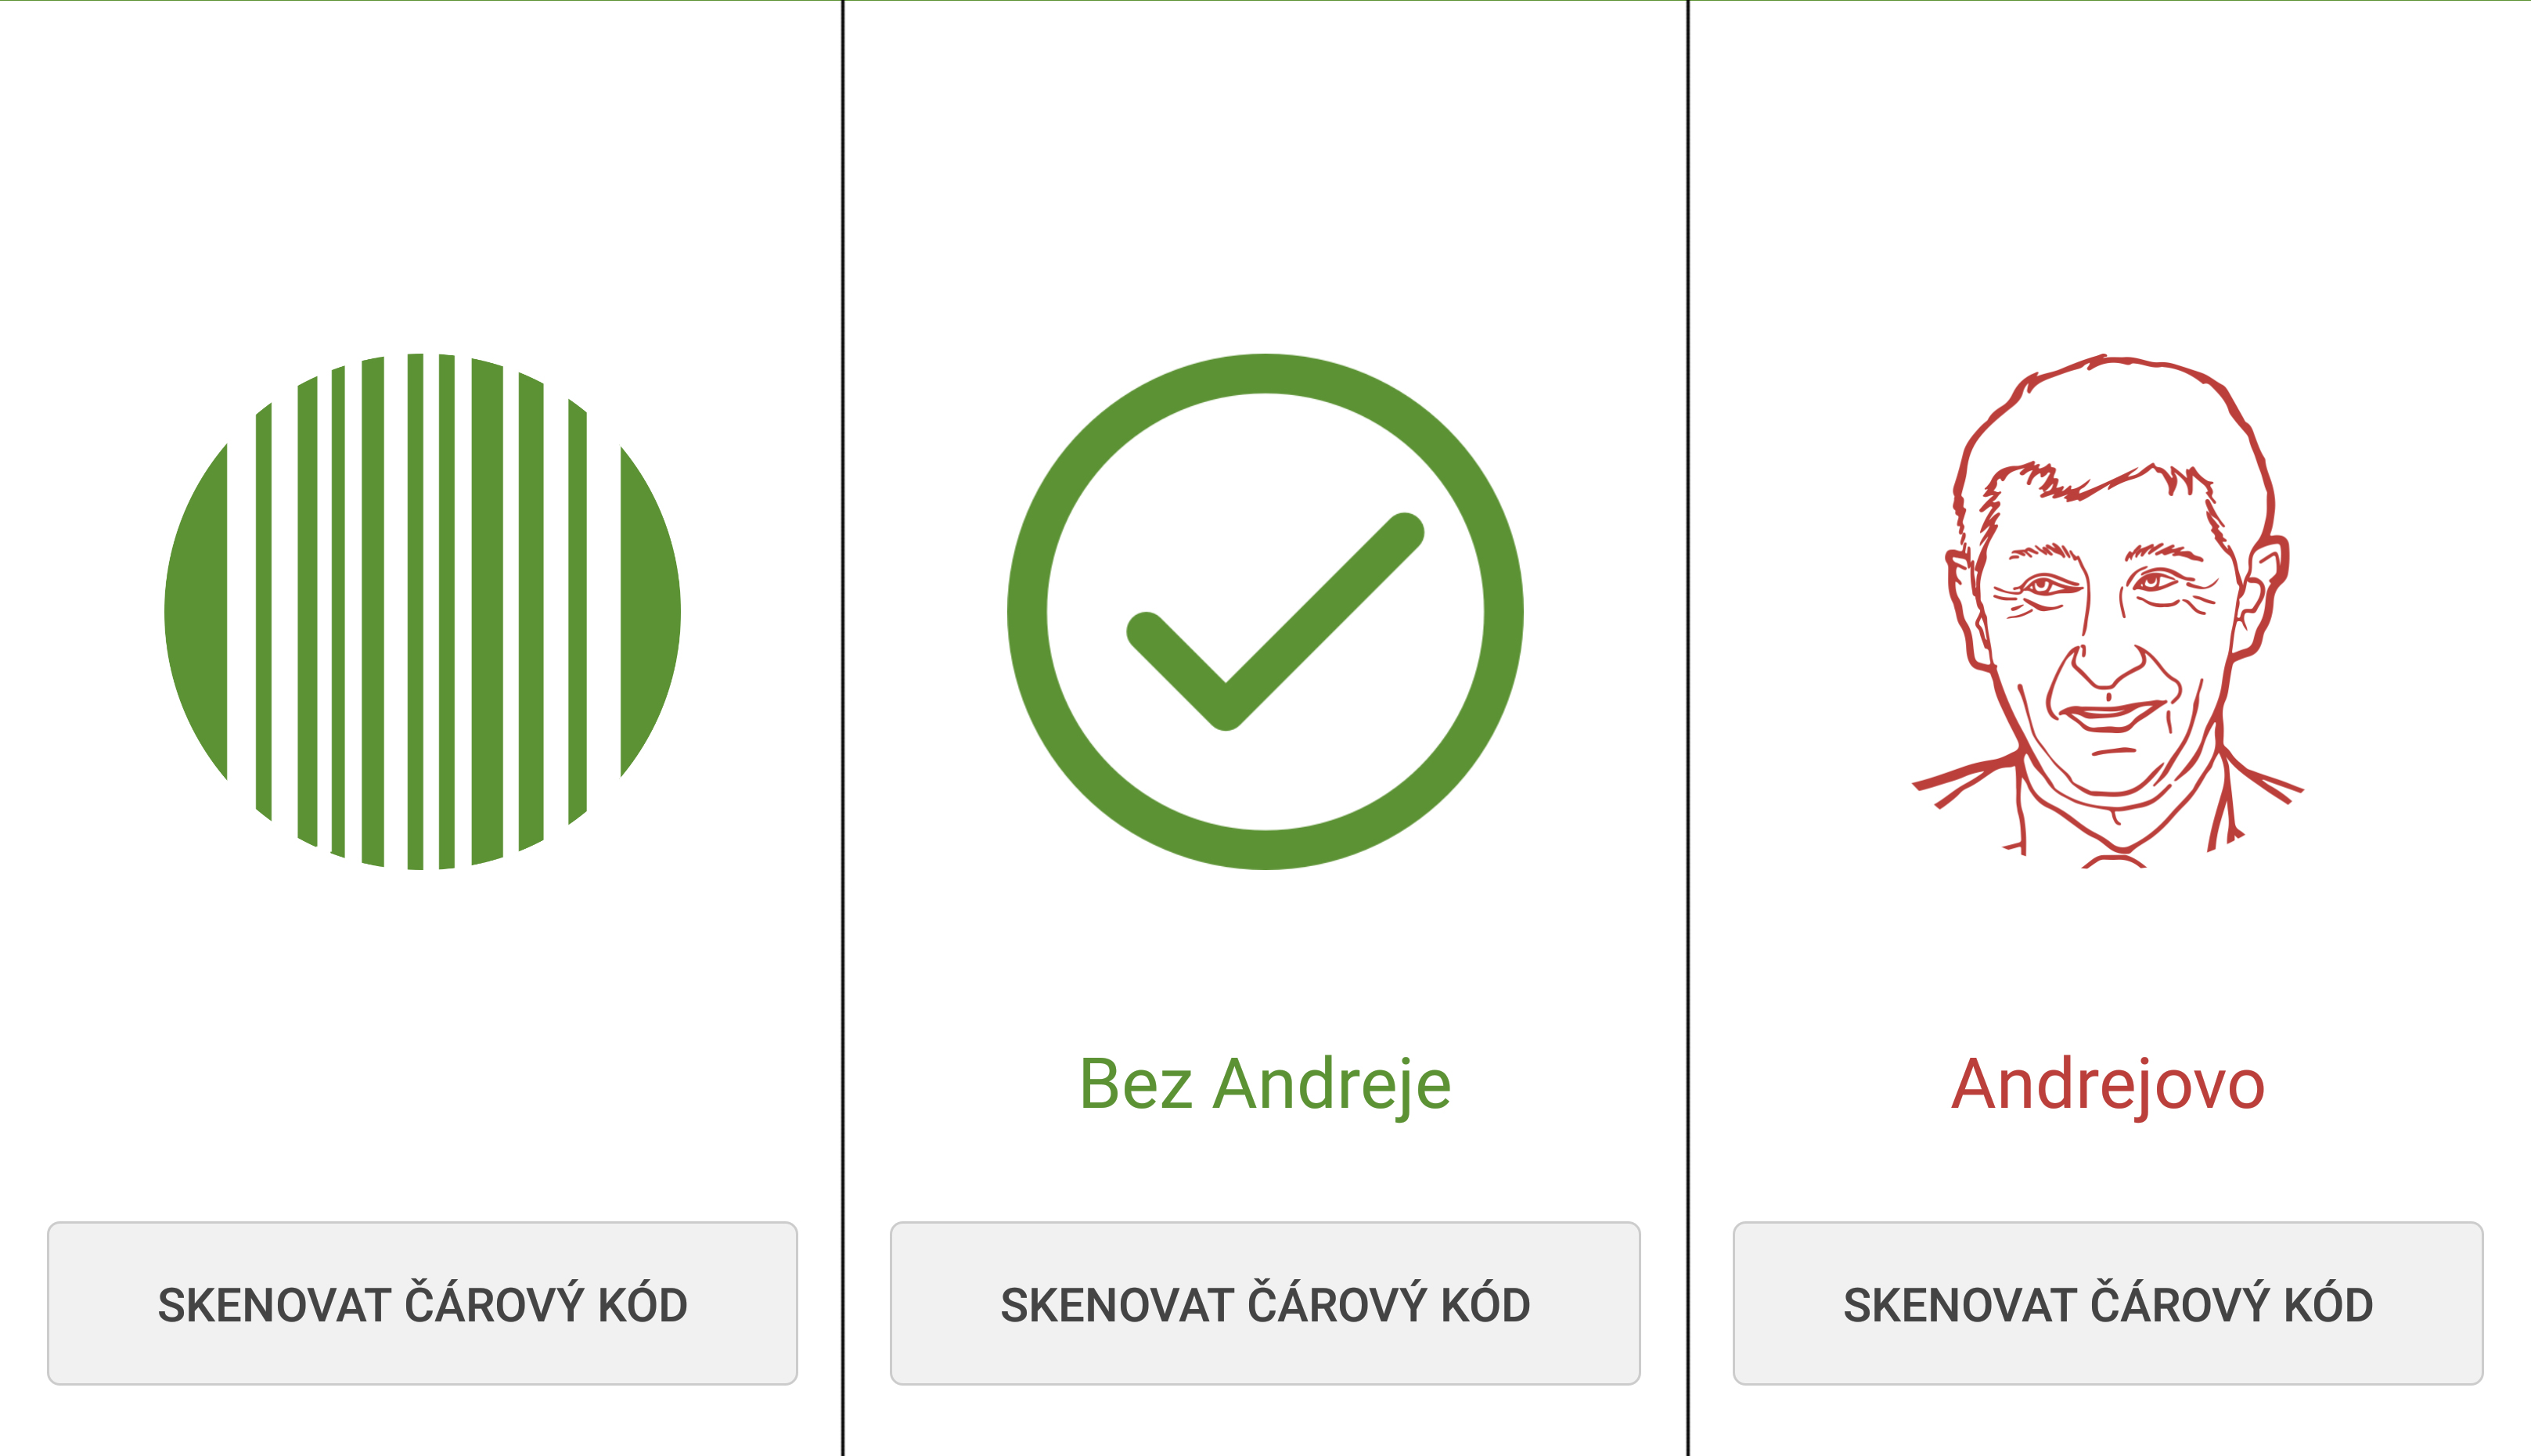
\includegraphics[width=.9\linewidth]{bez_andreje.jpg}
	\caption{\textit{Bez Andreje}'s homescreen and results}
	\label{fig:bezandreje}
\end{figure}
\subsection{UX}
It is obvious that the creator just focused on the app’s purpose and did not intend to use various design elements – the main screen consists of a big logo and a button for scanning the barcode. After successfuly scanning the barcode, the app informs the user whether the desired product is \textit{Babiš product} or not. In these situations the logo changes to a big green check icon or a red Ing. Andrej Babiš portrait (as showed in picture \ref{fig:bezandreje}).

%------------------------------------------------

\subsection{Quality of service} % Sub-section

Given the fact that the user interface is so simple, the most important part of the app is how it actually works rather than how it looks. Sometimes it happened to me that the \textit{Barcode Scanner} app did not catch a specific barcode, so \textit{Bez Andreje} left me stranded.

\newpage
When I first tried \textit{Bez Andreje} during the summer, I found a product, whose sub-supplier was a \textit{Babiš company} called \textit{Kostelecké uzeniny}, and as a result I got a big green check saying that this is not a \textit{Babiš product}.

Fortunately, while I was doing a research for this essay, I found this product again and the result was positive for \textit{Babiš company}. This means that the database is actually being updated from time to time. 

Nevertheless, in recent times, a lot of \textit{Babiš companies} started to mark their products with \textit{EAN8 barcode}, which is a clever way how to preserve the user from knowing whether he or she is buying a \textit{Babiš product}. \textit{Bez Andreje} does not deal with \textit{EAN8} codes at all. Any product that is not included in the database is not considered as a \textit{Babiš product}, so an user, who did not learn about \textit{EAN8} barcodes, can buy a \textit{Babiš product} while thinking that he or she buys a product that is safe.

\section{Bez Babiše}
\subsection{Overview}
The second app is also second at downloads count – 10k+ says \textit{Google Play} with the same rating of 4,2 stars. \textit{Bez Babiše} consumes 16 MB of phone’s storage, but it does not need a 3rd party app for barcode scanning. It also does not need a lot of permissions – just camera and internet access. The app works offline, it just recommends to connect to the internet from time to time to update the database.

Unfortunately the author did not respond to my e-mail, leaving me with no further information about used technologies.
\begin{figure}[h]
	\centering
	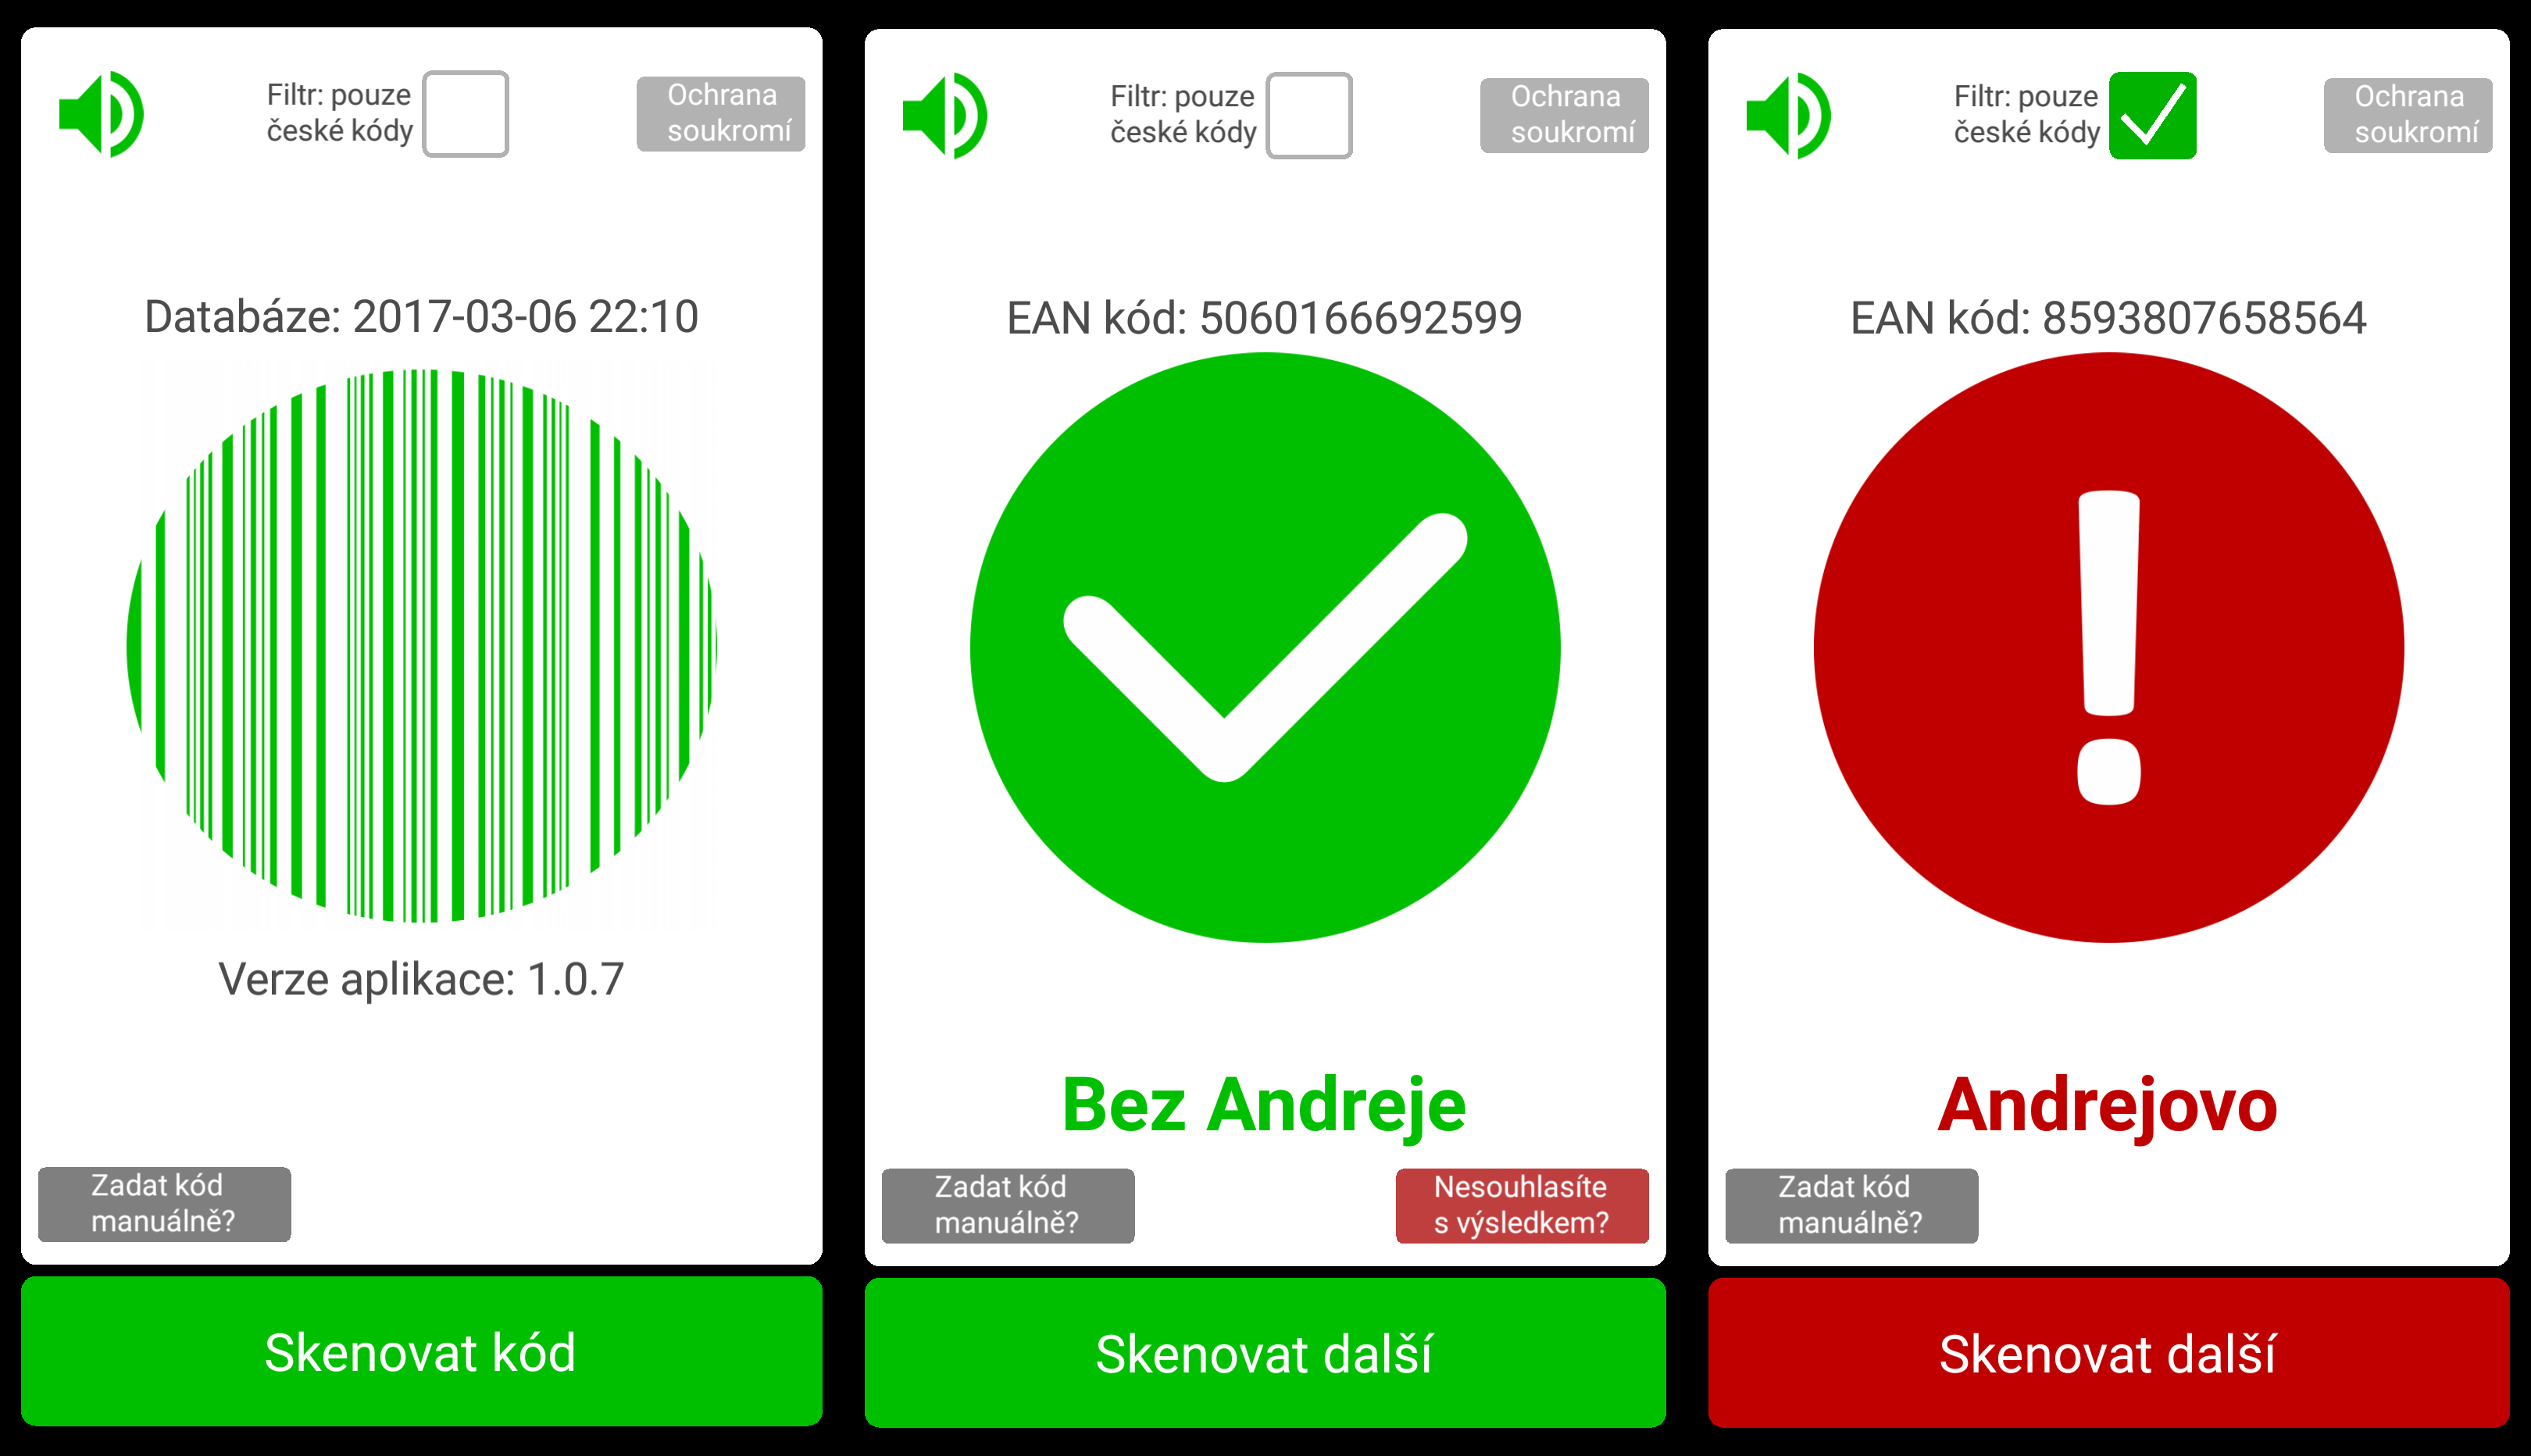
\includegraphics[width=.8\linewidth]{bez_babise.jpg}
	\caption{\textit{Bez Babiše}'s homescreen and results}
	\label{fig:bezbabise}
\end{figure}
\newpage
\subsection{UX}
The homescreen is very similar to \textit{Bez Andreje} – there is a big barcode logo in the middle of the screen and also a big button for scanning in the bottom of the screen. The user is informed about the version of the app and the database update timestamp. Moreover, the app has some additional functions. There is a button for assuring the user that the app just reads the barcode from the camera and does not use the photo for anything else but barcode recognition, another button for adding a barcode manually, a checkbox for turning on/off the sound and a checkbox for filtering only Czech barcodes. 

From an objective point of view I think that the visual part of the app could be a lot better – the worst impression make the additional buttons that seem to be placed randomly over the screen. 

After scanning, the app informs you with a big red exclamation mark if you have a \textit{Babiš product} in your hands, otherwise you see a big green check. At this point, you can disagree, which results into a information to the creators, who can check the company and add it to the database (picture \ref{fig:bezbabise}).

\subsection{Quality of service}
The barcode scanning works quite well – a situation where the app did not recognize a barcode has never occured to me. It also worked well when I was checking some products with a \textit{Babiš company} as a sub-supplier. What does not work so well are the database updates - right now the last database timestamp is a year and a half old. If that is true, the purpose of disagreeing with a result is a little bit pointless if the author became inactive.

\textit{Bez Babiše} deals with \textit{EAN8} codes by adding a third result option – unknown. Therefore, the user can not get a misinformation about an unrecognizable product (picture \ref{fig:bezbabise_unk}).

\begin{figure}[h]
	\centering
	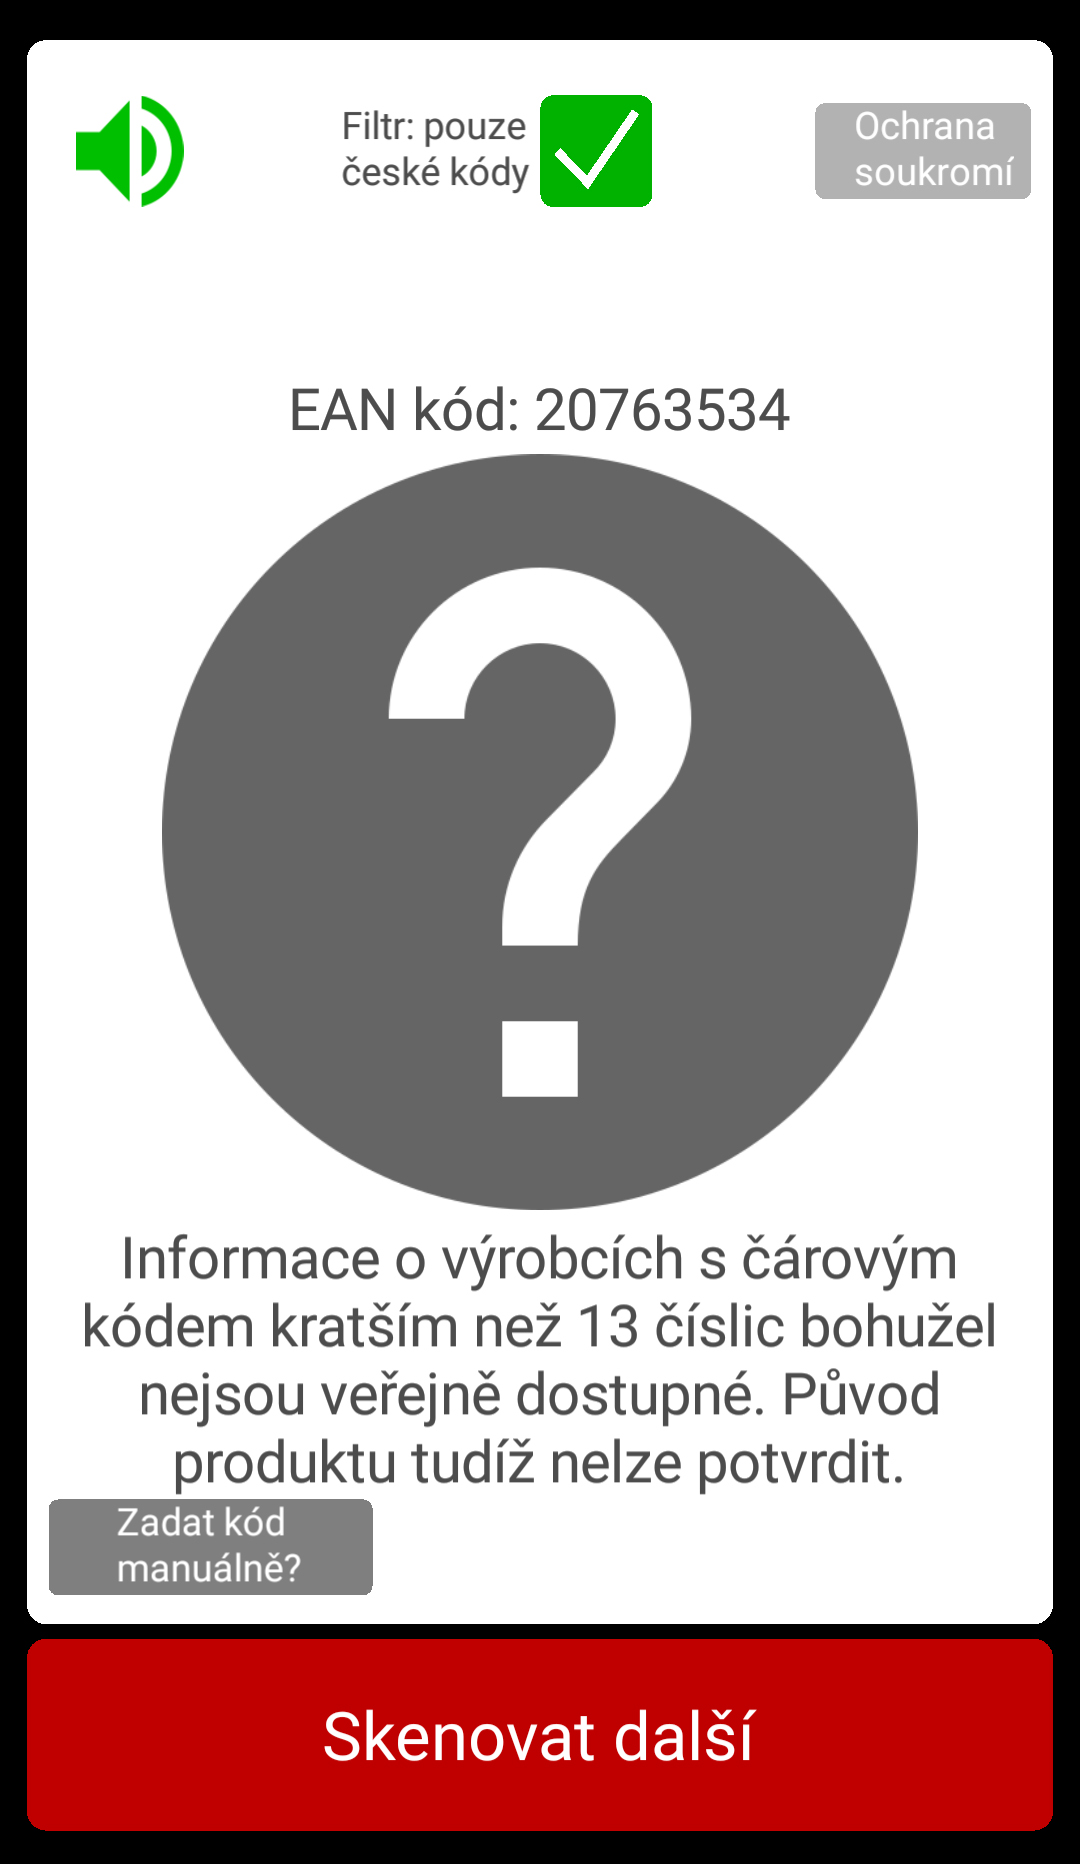
\includegraphics[width=0.25\linewidth]{bez_babise_unk.jpg}
	\caption{\textit{Bez Babiše} and dealing with \textit{EAN8} barcodes}
	\label{fig:bezbabise_unk}
\end{figure}

\section{Summary}
It is hard to say which one of the apps is better. \textit{Bez Andreje} looks better mainly because \textit{Bez Babiše} simply does not look very well (on the other hand, this is a very subjective point of view). However, \textit{Bez Babiše} adds more functionality – mainly adding the code manually and the possibility of disagreeing with the result. It also does not need a 3rd party app that requires a lot of permissions and can not mislead you to buy a \textit{Babiš product} if the product is unknown to the database.

The idea of the purpose is quite brilliant, given the fact that Ing. Andrej Babiš is very unpopular among a lot of Czech citizens, and therefore has a lot of potential. The question is whether the \textit{EAN8} codes will be used more and more, which would result into a slow death of these apps, unless they would somehow deal with this problem.



%----------------------------------------------------------------------------------------
%	BIBLIOGRAPHY
%----------------------------------------------------------------------------------------

\begin{thebibliography}{99} % Bibliography - this is intentionally simple in this template

\bibitem[1]{barcodes}
GS1 Czech Republic.
\newblock FAQ - čárové kódy.
\newblock \url{https://www.gs1cz.org/casto-kladene-dotazy/carove-kody}.
 
\end{thebibliography}

%----------------------------------------------------------------------------------------

\end{document}